\documentclass[12pt,letterpaper]{article}
\title{Attendance Project}
\author{G H Lathrom}

\usepackage{mystyle}
\usepackage{wasysym}
\usepackage{tensor}
\usepackage[all,cmtip]{xy}
%\usepackage{txfonts}
%\usepackage{stmaryrd}
\usepackage[dvips]{graphicx}
\usepackage[margin=1in,includehead]{geometry}
\usepackage{hyperref}

\newcommand{\lspan}{\operatorname{span}}
\newcommand{\Ob}{\operatorname{Ob}}
\newcommand{\id}{\operatorname{id}}
\newcommand{\diag}{\operatorname{diag}}
\newcommand{\SO}{\operatorname{SO}}
\newcommand{\Oth}{\operatorname{O}}
\newcommand{\supp}{\operatorname{supp}}
\newcommand{\invlim}{\varprojlim}

\renewcommand{\theenumi}{\roman{enumi}}
\renewcommand{\hat}{\widehat}

\begin{document}
\maketitle

%%%%%%%%%%%%%%%%%%%%%%%%%%%%%%%%%
%%% Header Style
%%%%%%%%%%%%%%%%%%%%%%%%%%%%%%%%%

\pagestyle{fancy}
\fancyhf{}
\lhead{\slshape Attendance Project}
\chead{}
\rhead{\slshape G H Lathrom}
\fancyfoot[C]{\thepage}
%\renewcommand{\chaptermark}[1]{\markboth{\chaptername \ 
%\thechapter. \ #1}{}} 
\renewcommand{\headrulewidth}{.5pt}
%%%%%%%%%%%%%%%%%%%%%%%%%%%%%%%%%
%\tableofcontents

\section{Overview}

This project explores the possibility of using image recognition with photos from student ids to perform automatic attendance checks.
The plan is to use OpenCV to process images and to write the code in C++.  
This is mainly because I want to write in a language other the Python in addition to speed being a factor.

\section{Basics of OpenCV}

The mathematical operation of \textbf{convolution} is a mathematical operation which takes in two functions, $f$ and $g$ and returns another function $f\ast g$ defined as
\begin{equation*}
    (f\ast g)(t) = \int_{-\infty}^\infty f(\tau)g(t-\tau)~d\tau
\end{equation*}
and satisfies the following properties:
\begin{enumerate}
    \item Commutativity:  $f\ast g = g \ast f$
    \item Associativity:  $f\ast(g\ast h) = (f\ast g)\ast h$
    \item Distributivity:  $f\ast (g+h) = f\ast g + f \ast h$
    \item Associativity of scalars:  $\alpha(f\ast g) = (\alpha f) \ast g$.
\end{enumerate}
Using the \textbf{distribution} or \textbf{generalized function}, the Dirac function, $\delta$, we can define an identity element
\begin{equation*}
    f\ast \delta = f
\end{equation*}
With respect to differentiation and integration we have
\begin{equation*}
    (f\ast g)' = f'\ast g = f\ast g' \buf{and}
    \int (f\ast g)~dx = \left( \int f~dx \right)\left( \int g~dx \right).
\end{equation*}
The discrete convolution of two functions is defined as
\begin{equation*}
    (f\ast g)(n) = \sum_{m=-\infty}^\infty f(m)g(n-m).
\end{equation*}
In the case of an image consisting of $n$-rows and $m$-columns, we may take the image as a function 
\begin{equation*}
    f:\left\{ 0, \ldots, n-1 \right\}\times\left\{ 0, \ldots, m-1 \right\} \ra \bb R
\end{equation*}
in the case a grey-scale image or
\begin{equation*}
    f:\left\{ 0, \ldots, n-1 \right\}\times\left\{ 0, \ldots, m-1 \right\} \ra \bb R^3
\end{equation*}
in the case of a color image with red-green-blue pixel triples.
We can extend these functions to functions of on all of $\bb Z$ in multiple ways, but here I mention a couple of common ways.
The first is to extend the function $f$ periodically to a function $\hat f$, that is we say
\begin{equation*}
    \hat f(i,j) = f(i \hspace{-1ex}\pmod n, ~j\hspace{-1ex}\pmod m)
\end{equation*}
where we have taken the standard representation sets $\left\{ 0, \ldots, n-1 \right\}$ and $\left\{ 0, \ldots, m-1 \right\}$.
This would take an image to periodic image as shown in Figure \ref{fig:periodic}.
Another extension is to simply make the values zero outside of the original image values as
\begin{equation*}
    \hat f(i,j) = 
    \begin{cases}
        f(i,j), & (i,j) \in \left\{ 0,\ldots,n-1 \right\}\times\left\{ 0,\ldots,m-1 \right\} \\
        0 & \textup{otherwise}
    \end{cases}
\end{equation*}
\begin{figure}[htpb]
    \centering
    \begin{minipage}[c]{.4\textwidth}
        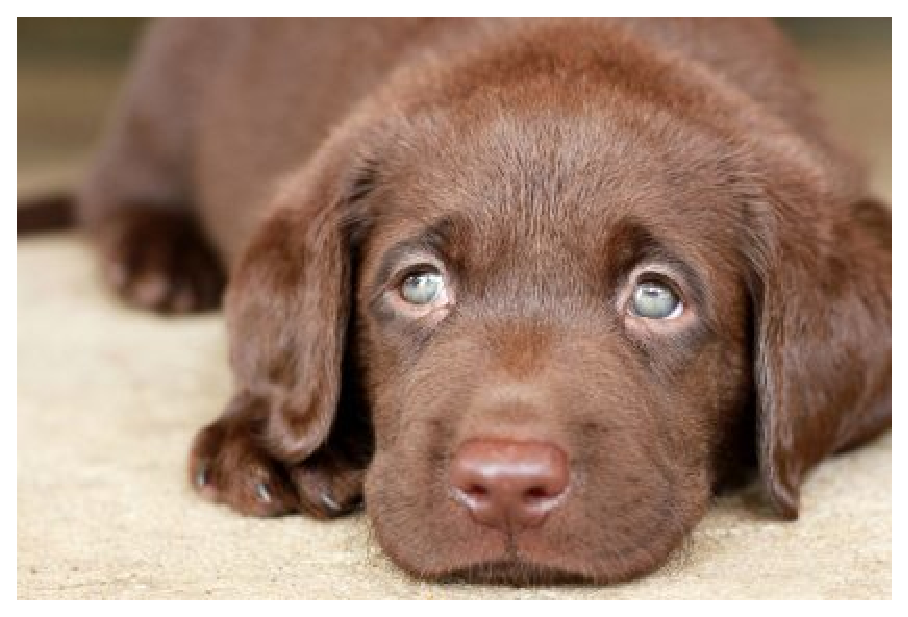
\includegraphics[width=\textwidth]{images/lab}
    \end{minipage}
    \qquad $\longrightarrow$ \qquad
    \begin{minipage}[c]{.4\textwidth}
        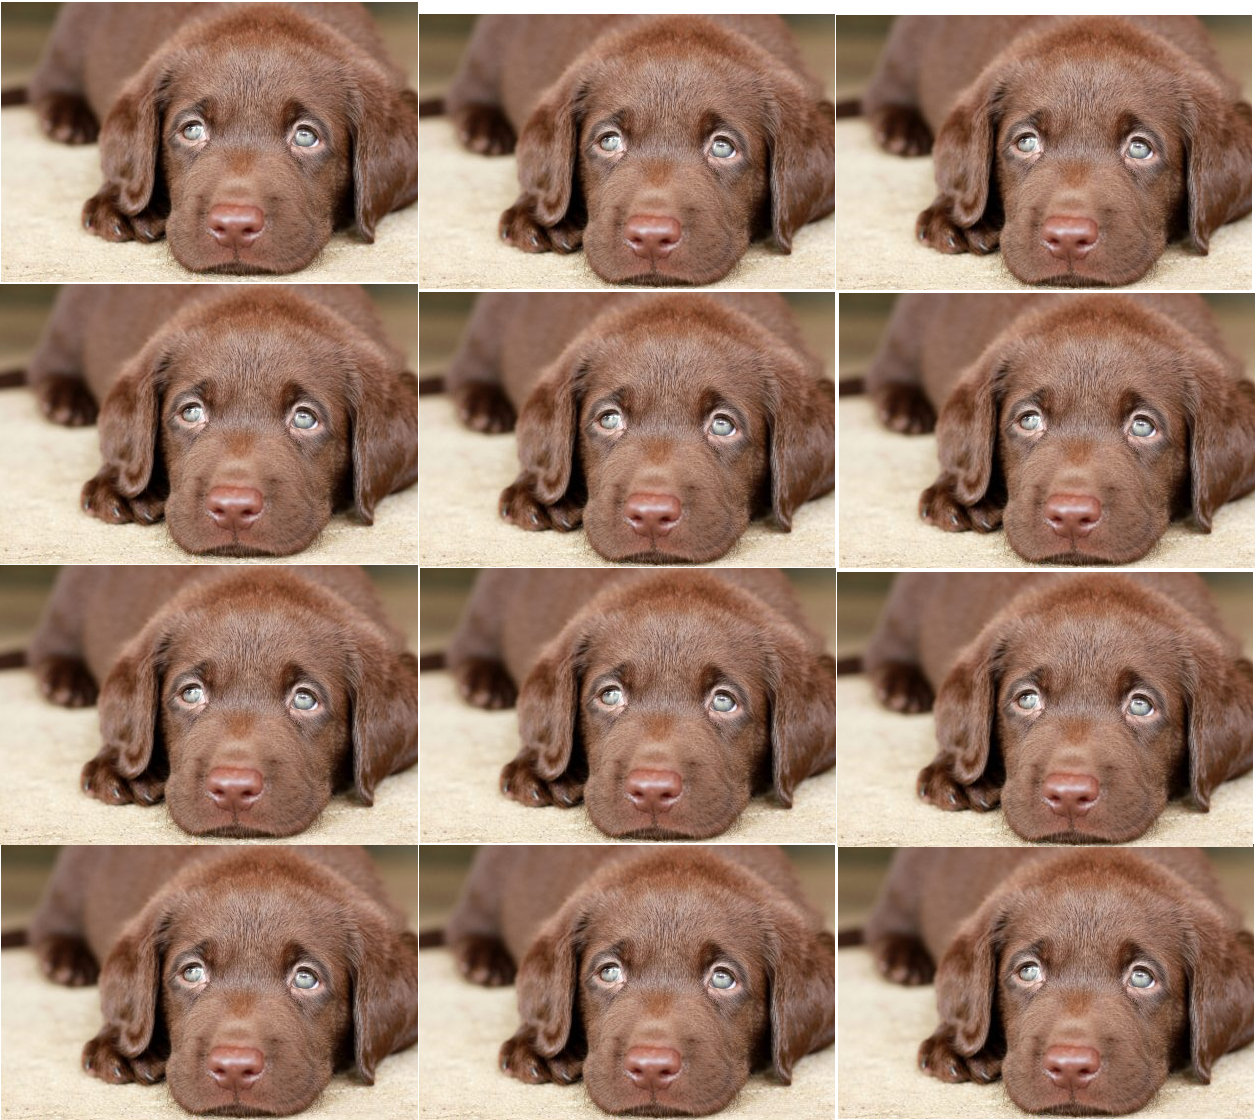
\includegraphics[width=\textwidth]{images/lab2}
    \end{minipage}
    \caption{Periodic Boundary}
    \label{fig:periodic}
\end{figure}




\cite{babyrudin}


\bibliographystyle{amsalpha}
\bibliography{/home/grant/texmf/tex/latex/thebibliography}

\end{document}
